\section{Sistemas no Chua evaluados como referencias dinámicas}
\label{sec:nonchua-dynamic-benchmarks}

\subsection{Clasificación homogénea de los casos ejecutados}

Los sistemas no Chua ejecutados se dividen en dos grupos. El primero contiene
los casos enteros en los que la localización produjo un conjunto recurrente y
se completaron pruebas de periodicidad o caos, vecindades de los equilibrios y
comparación independiente. Los controles de estabilidad numérica se consignan
sólo cuando existe el artefacto canónico correspondiente. El segundo contiene
referencias fraccionarias empleadas para evaluar algoritmos de exponentes de
Lyapunov. En estas últimas no se ejecutó una localización por continuación ni un
análisis de vecindades; por consiguiente, sus resultados caracterizan el método
numérico y no establecen ocultedad.

\begingroup
\small
\setlength{\tabcolsep}{3pt}
\begin{longtable}{@{}L{0.19\linewidth}L{0.16\linewidth}L{0.18\linewidth}L{0.40\linewidth}@{}}
\caption{Cobertura homogénea de los sistemas no Chua ejecutados.}
\label{tab:nonchua-unified-evidence}\\
\toprule
Sistema & Orden & Conjunto o diagnóstico & Resultado numérico y alcance\\
\midrule
\endfirsthead
\toprule
Sistema & Orden & Conjunto o diagnóstico & Resultado numérico y alcance\\
\midrule
\endhead
Kalman--Fitts & \(1\) & Ciclo límite estable &
\(T=11.9169960\); 48 condiciones alrededor del único equilibrio, sin contactos
con el ciclo; reproducción independiente en Julia.\\
MAVPD, \(\xi=3.1\) & \(1\) & Ciclo externo estable &
\(T=0.493177986749\), \(K_{0-1}=4.40086\times10^{-4}\), espectro
\((-0.0017614,-0.3887396,-51.1886634)\); 108 condiciones alrededor de tres
equilibrios, sin contactos; comparación Python--Julia.\\
MAVPD, \(\xi=2.85\) & \(1\) & Candidato caótico &
\(\widehat\lambda_1=\MAVPDChaosLEOne\), \(D_{KY}=\MAVPDChaosKY\); sección de
Poincaré y prueba 0--1 sobre retornos; \MAVPDChaosTotalProbes{} condiciones de
vecindad y controles dirigidos, sin contactos; comparación Python--Julia.\\
PLL lead--lag & \(1\) & Ciclo corrido estable &
\(T=\PLLPythonStablePeriod\), multiplicador
\(\PLLPythonStableMultiplier\); 96 condiciones alrededor de dos equilibrios,
sin contactos; reproducción independiente en Julia.\\
Lorenz estándar & \(q=0.985\) & Referencia variacional &
Tres exponentes finito-temporales dentro de la tolerancia publicada; no se
realizó una búsqueda de atractor oculto.\\
Rabinovich--Fabrikant, \(b=0.98\) & \(q=0.999\) & Referencia variacional &
Dos exponentes dentro de tolerancia y discrepancia \(0.2525353\) en
\(\lambda_3\); no se realizó una búsqueda de atractor oculto.\\
Jerk exponencial & conmensurable e inconmensurable & Dinámica clonada &
Ocho filas evaluadas: cuatro conservan el patrón de signos y cuatro presentan
discrepancias; sin prueba de vecindades.\\
Sistema financiero & conmensurable e inconmensurable & Dinámica clonada &
Ocho filas evaluadas: cinco coincidencias cuantitativas, dos de signos y una
discrepante; sin prueba de vecindades.\\
Sistema four-wing & conmensurable e inconmensurable & Dinámica clonada &
Ocho filas evaluadas: cinco coincidencias cuantitativas y tres discrepantes;
sin prueba de vecindades.\\
\bottomrule
\end{longtable}
\endgroup

\subsection{Formulación y evidencia de los cuatro candidatos enteros}

En cada candidato se distinguen la declaración dinámica, el análisis local, la
ruta de localización y el resultado numérico. Las ausencias de contacto se
refieren exclusivamente a las condiciones iniciales declaradas y no constituyen
una demostración global de separación de cuencas.

\subsubsection{Kalman--Fitts de cuarto orden}

\paragraph{Modelo y estabilidad local.}
Con \(m_1=0.9\), \(m_2=1.1\), \(\beta=0.03\) y
\(\varepsilon=0.01\), el sistema de Kuznetsov et
al.~\cite{kalman2019} se escribe exactamente en forma de Lur'e como
\begin{equation}
 \dot X=AX+b\tanh\!\left(\frac{c^{\mathsf T}X}{\varepsilon}\right),
 \qquad b=e_4,\qquad c=-e_3,
 \label{ncbench:eq:kalman-lure}
\end{equation}
donde \(A\) es la matriz compañera del polinomio
\begin{equation}
 \begin{gathered}
  \begin{aligned}
   p_A(s)&=\bigl[s^2+2\beta s+(m_1^2+\beta^2)\bigr]
            \bigl[s^2+2\beta s+(m_2^2+\beta^2)\bigr]\\
   &=s^4+0.12s^3+2.0254s^2+0.121308s+0.98191881,
  \end{aligned}\\[0.6em]
  A=\begin{pmatrix}
   0&1&0&0\\0&0&1&0\\0&0&0&1\\
   -0.98191881&-0.121308&-2.0254&-0.12
  \end{pmatrix}.
 \end{gathered}
 \label{ncbench:eq:kalman-matrix}
\end{equation}
El único equilibrio es \(E_0=0\). Su Jacobiano
\(J(E_0)=A+\varepsilon^{-1}bc^{\mathsf T}\) tiene espectro
\begin{equation}
 \operatorname{spec}J(E_0)=
 \{-0.05941105\pm10.10010422i,
   -0.0005889505\pm0.09810623i\},
 \label{ncbench:eq:kalman-spectrum}
\end{equation}
por lo que \(E_0\) es localmente asintóticamente estable.

\paragraph{Localización y configuración.}
La transferencia derivada de~\eqref{ncbench:eq:kalman-lure} es
\(W(s)=-s^2/p_A(s)\). Su cierre imaginario positivo da
\(\omega_0=1.005435229142\) y exige
\(k=-0.043168701157\), mientras que la función descriptiva de la tangente
hiperbólica toma valores en \((0,100)\) para amplitud positiva. La ruta directa
queda, por tanto, descartada por incompatibilidad de signo. La alternativa
reemplaza temporalmente la no linealidad por
\(\operatorname{sign}(c^{\mathsf T}X)\), itera el mapa exacto de cruces de
\(c^{\mathsf T}X=0\) y obtiene, tras 135 iteraciones del mapa de cruces, un
retorno de periodo dos con
\begin{equation}
 X_{\mathrm{sw}}=(0.212347571803,-1.671123727247,0,
 1.478087383043)^{\mathsf T}.
 \label{ncbench:eq:kalman-switching-seed}
\end{equation}
Desde esa semilla se continúa
\((1-\lambda)\operatorname{sign}\sigma+
\lambda\tanh(\sigma/\varepsilon)\) en 51 nodos
\(\lambda=0,0.02,\ldots,1\). Cada nodo usa RK4 con \(h=0.01\), transitorio
100 y ventana conservada 20; la corrida final emplea transitorio 300 y ventana
300.

\paragraph{Resultado y alcance.}
La sección de Poincaré da un ciclo estable con periodo medio
\(T=11.9169960234\). El espectro finito
\((-0.00283635,-0.02423392,-0.03056980,-0.03988642)\) es compatible con un
exponente que converge lentamente a cero y tres exponentes negativos. Se
integraron 48 condiciones alrededor de \(E_0\), con radios
\(10^{-5},10^{-4},10^{-3},10^{-2}\) y 12 muestras por radio: 40 terminaron
en el equilibrio, ocho quedaron acotadas y no triviales, y ninguna contactó
el ciclo. La implementación independiente reprodujo el retorno de periodo dos,
las 48 clasificaciones y el ciclo con periodo \(11.9169379538\); la diferencia
de periodos fue \(5.81\times10^{-5}\). La matriz canónica de estabilidad
numérica combina DOP853 estándar y ajustado con RK4 a
\(h=0.01\) y \(h=0.005\), cada uno en horizontes 300 y 600. Las ocho
configuraciones fueron consistentes: el error relativo del periodo quedó entre
\(4.87\times10^{-6}\) y \(6.11\times10^{-6}\), el error máximo de retorno
entre \(4.18\times10^{-4}\) y \(1.44\times10^{-3}\), y la distancia
normalizada entre nubes entre \(2.03\times10^{-4}\) y
\(9.24\times10^{-4}\). Este control sustenta persistencia numérica
finito-temporal bajo esas configuraciones, no periodicidad, atracción u ocultedad
globales.

\subsubsection{MAVPD periódico con \texorpdfstring{\(\xi=3.1\)}{xi=3.1}}

\paragraph{Modelo y estabilidad local.}
El sistema autónomo de Van der Pol--Duffing modificado
\cite{matouk2023} es
\begin{equation}
 \begin{aligned}
  \dot y_1&=\delta\gamma y_1+\delta y_2-\delta y_1^3,\\
  \dot y_2&=y_1-\xi y_2-y_3,\\
  \dot y_3&=\rho y_2,
 \end{aligned}
 \qquad
 P=\begin{pmatrix}
 \delta\gamma&\delta&0\\1&-\xi&-1\\0&\rho&0
 \end{pmatrix},\quad
 b=\begin{pmatrix}-\delta\\0\\0\end{pmatrix},\quad
 c=e_1,\quad \psi(\sigma)=\sigma^3.
 \label{ncbench:eq:mavpd-lure}
\end{equation}
La descomposición \(\dot y=Py+b\psi(c^{\mathsf T}y)\) es exacta. Para
\(\gamma>0\), sus equilibrios y Jacobiano son
\begin{equation}
 E_0=(0,0,0),\qquad
 E_\pm=(\pm\sqrt{\gamma},0,\pm\sqrt{\gamma}),\qquad
 J(y)=\begin{pmatrix}
 \delta(\gamma-3y_1^2)&\delta&0\\
 1&-\xi&-1\\0&\rho&0
 \end{pmatrix}.
 \label{ncbench:eq:mavpd-equilibria-jacobian}
\end{equation}
En \(E_\pm\), el polinomio característico es
\begin{equation}
 p_\pm(\mu)=\mu^3+(\xi+2\delta\gamma)\mu^2
 +(\rho-\delta+2\delta\gamma\xi)\mu+2\delta\gamma\rho.
 \label{ncbench:eq:mavpd-local-polynomial}
\end{equation}
Para \((\gamma,\delta,\rho,\xi)=(0.1,100,200,3.1)\), \(E_0\) posee un
autovalor real positivo y \(E_\pm\) un par complejo con parte real positiva;
los tres equilibrios son inestables.

\paragraph{Localización y configuración.}
La transferencia y la función descriptiva derivadas de
\eqref{ncbench:eq:mavpd-lure} son
\begin{equation}
 G(s)=\frac{\delta(s^2+\xi s+\rho)}
 {s^3+(\xi-\delta\gamma)s^2+
 (\rho-\delta-\delta\gamma\xi)s-\delta\gamma\rho},
 \qquad \mathcal N(a)=\frac{3a^2}{4}.
 \label{ncbench:eq:mavpd-transfer}
\end{equation}
Con \(z=\omega^2\), la condición de cierre se reduce a
\(z^2-290.39z+20000=0\). Sin barrido de frecuencias aparecen las ramas
\begin{equation}
 \begin{array}{c|ccc}
 j&\omega_j&k_j&a_j\\ \hline
 0&10.5975230311&0.1397015948&0.4315886851\\
 1&13.3447557342&0.3518790503&0.6849613618
 \end{array}
 \label{ncbench:eq:mavpd-periodic-branches}
\end{equation}
y se integran ambas fases, \(0\) y \(\pi\), en 21 nodos
\(\lambda=0,0.05,\ldots,1\). La continuación usa RK4 con \(h=0.002\),
transitorio 20 y cola 10; el refinamiento final usa DOP853 con
\((\mathrm{rtol},\mathrm{atol})=(2\times10^{-11},2\times10^{-13})\), paso
máximo \(0.005\), transitorio 600 y ventana 1200. La rama 0 produce los dos
ciclos internos simétricos y la rama 1 el ciclo externo, seleccionado por su
mayor extensión de estado.

\paragraph{Resultado y alcance.}
La sección \(y_2=0\), con cruce positivo, retuvo 2433 retornos y dio
\begin{equation}
 \begin{aligned}
  T&=0.493177986749,\\
  K_{0-1}&=4.4008572555\times10^{-4},\\
  \widehat\lambda&=(-0.00176137,-0.38873958,-51.18866339).
 \end{aligned}
 \label{ncbench:eq:mavpd-periodic-results}
\end{equation}
Los 108 sondeos, definidos por tres equilibrios, tres radios
\(10^{-5},10^{-3},10^{-2}\) y 12 direcciones, usaron \(h=0.005\),
transitorio 180 y cola 80. Cincuenta y cuatro terminaron en cada ciclo interno
y ninguno contactó el ciclo externo. La reproducción independiente obtuvo
\(T=0.493178150753\), coincidió en las 108 asignaciones y tampoco registró
contactos con el ciclo externo. El resultado sostiene un ciclo externo oculto
sólo bajo el protocolo finito declarado.

\subsubsection{MAVPD caótico con \texorpdfstring{\(\xi=2.85\)}{xi=2.85}}

\paragraph{Modelo y estabilidad local.}
Se conserva la realización~\eqref{ncbench:eq:mavpd-lure}, pero el punto
numérico localizado es
\begin{equation}
 (\xi,\gamma,\delta,\rho)=
 (2.85,0.153803798399491,100,200).
 \label{ncbench:eq:mavpd-chaos-parameters}
\end{equation}
Este valor de \(\gamma\) no es un parámetro publicado. Los equilibrios son
\(E_0=0\) y
\(E_\pm=(\pm0.392178273747,0,\pm0.392178273747)\). El Jacobiano de
\eqref{ncbench:eq:mavpd-equilibria-jacobian} da
\begin{equation}
 \begin{aligned}
  \operatorname{spec}J(E_0)&=
  \{18.49014976,-2.97988496\pm12.54923270i\},\\
  \operatorname{spec}J(E_\pm)&=
  \{-33.49198782,-0.05938593\pm13.55310787i\}.
 \end{aligned}
 \label{ncbench:eq:mavpd-chaos-spectra}
\end{equation}
Por tanto, \(E_0\) es inestable y \(E_\pm\) son localmente asintóticamente
estables.

\paragraph{Localización y configuración.}
En el punto base \((\xi,\gamma)=(3.1,0.1)\), las dos ramas directas de
\eqref{ncbench:eq:mavpd-periodic-branches} produjeron
\(\widehat\lambda_1=-0.00125057\) y \(-0.00299485\), por debajo del umbral
finito \(0.02\). Este fallo activa una continuación alternativa: se selecciona
la rama 0 por su menor frecuencia, se transporta el estado desde
\(\xi=3.10\) hasta \(2.85\) en pasos de \(-0.01\), y después se varía
\(\gamma\) respecto de la frontera de Routh--Hurwitz
\begin{equation}
 \xi g^2+(\xi^2-\delta)g+\xi(\rho-\delta)=0,
 \qquad g=2\delta\gamma.
 \label{ncbench:eq:mavpd-hopf-boundary}
\end{equation}
La raíz alta es \(\gamma_H=0.143803798399491\). Entre los desplazamientos
declarados, la regla selecciona \(\gamma=\gamma_H+0.010\): fue el mayor
desplazamiento ensayado con exponente máximo mayor que \(0.5\), cero contactos
preliminares desde \(E_0\), cero ambigüedades y cero fallos. Esta igualdad sólo
determina una frontera candidata de cruce imaginario; no verifica las
condiciones completas de una bifurcación de Hopf.

La trayectoria estricta usa DOP853 hasta \(t=900\), descarta 300, muestrea cada
\(0.02\) y fija \((\mathrm{rtol},\mathrm{atol})=(2\times10^{-11},
2\times10^{-13})\) con paso máximo \(0.01\). El sistema variacional usa
transitorio 300, acumulación 1200 y QR cada \(0.5\), con tolerancias
\((2\times10^{-12},2\times10^{-14})\).

\paragraph{Resultado y alcance.}
Los diagnósticos finito-temporales son
\begin{equation}
 \widehat\lambda=(0.7133503985,-0.0009058833,-20.9236249563),
 \qquad D_{KY}=2.0340497651.
 \label{ncbench:eq:mavpd-chaos-results}
\end{equation}
La sección \(y_2=0\) contiene 1174 cruces no duplicados; la prueba 0--1
sobre sus dos coordenadas da medianas \(0.9985162431\) y \(0.9984323397\).
El protocolo final comprende 108 condiciones alrededor de los tres
equilibrios y cuatro controles sobre ambos signos de la dirección inestable de
\(E_0\): las 112 trayectorias terminaron en equilibrios, sin contactos,
ambigüedades ni fallos. La matriz de estabilidad numérica registró consistencia
al variar integrador, paso y horizonte; la memoria no es aplicable al sistema
entero. Una implementación independiente recuperó los mismos parámetros y las
112 decisiones; obtuvo
\(\widehat\lambda=(0.6938035753,0.0017936287,-20.9005938240)\), 1175 cruces y
\(K=0.9971592730\). La clasificación resultante es candidato caótico oculto bajo
las vecindades ensayadas, no una prueba global de caos u ocultedad.

\subsubsection{PLL bifásico con filtro lead--lag}

\paragraph{Modelo, cilindro y estabilidad local.}
El modelo de Bianchi et al.~\cite{pll2015} es
\begin{equation}
 \dot x=-\frac{x}{T}+\frac{\tau_1}{2T}\sin\theta,
 \qquad
 \dot\theta=\omega_\Delta-\frac{Lx}{T}
 -\frac{\tau_2L}{2T}\sin\theta,
 \qquad T=\tau_1+\tau_2,
 \label{ncbench:eq:pll-original}
\end{equation}
con \((\tau_1,\tau_2,L,\omega_\Delta)=(0.0448,0.0185,500,178.9)\).
Los equilibrios bloqueados satisfacen
\begin{equation}
 x_e=0.01602944,\qquad
 \theta_f=0.797482699882,\qquad
 \theta_s=2.344109953708.
 \label{ncbench:eq:pll-equilibria}
\end{equation}
Al trasladar \(u=x-x_e\), \(v=\theta-\theta_f\), se obtiene la forma T1
exacta
\begin{equation}
 \begin{pmatrix}\dot u\\\dot v\end{pmatrix}
 =P\begin{pmatrix}u\\v\end{pmatrix}+b\phi(v),\qquad
 P=\begin{pmatrix}-1/T&0\\-L/T&0\end{pmatrix},\quad
 b=\begin{pmatrix}\tau_1/(2T)\\-\tau_2L/(2T)\end{pmatrix},
 \quad \phi(v)=\sin(\theta_f+v)-\sin\theta_f.
 \label{ncbench:eq:pll-lure}
\end{equation}
El estado pertenece a \(\mathbb R\times S^1\); las diferencias angulares se
evalúan módulo \(2\pi\). En las coordenadas trasladadas,
\(E_f=(0,0)\) y \(E_s=(0,1.546627253827)\), y
\begin{equation}
 J(u,v)=\begin{pmatrix}
 -1/T&\tau_1\cos(\theta_f+v)/(2T)\\
 -L/T&-\tau_2L\cos(\theta_f+v)/(2T)
 \end{pmatrix}.
 \label{ncbench:eq:pll-jacobian}
\end{equation}
Los espectros son
\begin{align}
 \operatorname{spec}J(E_f)&=
 \{-33.41714171\pm40.52189661\ii\},\\
 \operatorname{spec}J(E_s)&=\{-37.78074660,73.01945339\}.
\end{align}
El primero es un foco estable y el segundo una silla.

\paragraph{Localización y configuración.}
La transferencia normalizada de la forma trasladada es
\begin{equation}
 G(s)=-\frac{L}{2}\frac{1+\tau_2s}{s(1+Ts)}.
 \label{ncbench:eq:pll-transfer}
\end{equation}
La expresión algebraica satisface \(\operatorname{Im}G(i\omega)>0\) para todo
\(\omega>0\); no existe un cruce directo compatible con una función
descriptiva estática real y acotada. Al eliminar \(x\) y definir
\(y=\dot\theta\), la ruta alternativa usa
\begin{equation}
 T\dot y=\omega_\Delta-\frac{L}{2}\sin\theta
 -\left(1+\frac{\tau_2L}{2}\cos\theta\right)y.
 \label{ncbench:eq:pll-andronov}
\end{equation}
Para \(L=0\) se conoce analíticamente la solución corrida; su órbita se
continúa hasta \(L=500\) en 101 valores. El mapa de retorno emplea la sección
\(\theta=0\pmod{2\pi}\), tolerancias
\((\mathrm{rtol},\mathrm{atol})=(2\times10^{-11},2\times10^{-13})\) y paso
angular máximo \(0.02\). Las condiciones publicadas se reservan para una
regresión posterior y no intervienen en la localización.

\paragraph{Resultado y alcance.}
En \(L=500\), el mapa localiza un ciclo corrido estable y su separatriz
periódica inestable:
\begin{equation}
 \begin{array}{c|cc}
 &T&\text{multiplicador}\\ \hline
 \text{ciclo estable}&0.0826766624974002&0.81720414315349\\
 \text{separatriz}&0.108541779638197&1.4411073306967
 \end{array}
 \label{ncbench:eq:pll-cycle-results}
\end{equation}
Los errores de retorno cilíndrico son \(2.68\times10^{-15}\) y
\(6.18\times10^{-14}\), respectivamente. El sondeo usa los dos equilibrios,
cuatro radios \(10^{-5},10^{-4},10^{-3},10^{-2}\) y 12 muestras por radio:
las 96 condiciones terminaron en el foco y ninguna alcanzó el ciclo. La
implementación independiente reprodujo el periodo y multiplicador estables
como \(0.0826766624969991\) y \(0.817204143145181\), coincidió en las 96
decisiones y mantuvo distancias cilíndricas máximas de
\(3.28\times10^{-12}\) para el ciclo y \(1.82\times10^{-11}\) para la
separatriz. La evidencia de ocultedad queda restringida a las vecindades
cilíndricas finitas ensayadas.

\subsection{Sistema variacional y exponentes finito-temporales}

Danca y Kuznetsov~\cite{DancaKuznetsov2018Lyapunov} consideran el sistema
extendido
\begin{equation}
 {}^{\mathrm C}D^q X=f(X),\qquad
 {}^{\mathrm C}D^q\Phi=J_f(X)\Phi,\qquad \Phi(0)=I.
 \label{ncbench:eq:variational}
\end{equation}
Después de cada intervalo de normalización, las columnas de \(\Phi\) se
ortogonalizan y se acumulan los logaritmos de las normas. Para \(K\) intervalos
de longitud \(T_R\), el estimador es
\begin{equation}
 \widehat\lambda_i(KT_R)=\frac{1}{KT_R}
 \sum_{k=1}^{K}\log r_{ii}^{(k)},
 \label{ncbench:eq:benettin}
\end{equation}
donde \(r_{ii}^{(k)}\) son las entradas diagonales positivas producidas por la
ortogonalización. Las corridas reproducidas emplean Adams--Bashforth--Moulton
(ABM) por bloques y Gram--Schmidt. El reinicio entre bloques reproduce el
procedimiento publicado, pero no equivale a una integración de Caputo con
memoria global continua.

\subsection{Lorenz estándar fraccionario, \texorpdfstring{\(q=0.985\)}{q=0.985}}

\subsubsection*{Modelo, realización algebraica y equilibrios}

El caso evaluado es
\begin{equation}
\begin{aligned}
 {}^{\mathrm C}D^q x&=\sigma(y-x),\\
 {}^{\mathrm C}D^q y&=\rho x-y-xz,\\
 {}^{\mathrm C}D^q z&=xy-\beta z,
\end{aligned}
\qquad
(\sigma,\rho,\beta,q)=\left(10,200,\frac83,0.985\right).
\label{ncbench:eq:lorenz-standard}
\end{equation}
Una realización polinómica exacta es
\begin{equation}
 A=\begin{pmatrix}-\sigma&\sigma&0\\ \rho&-1&0\\0&0&-\beta\end{pmatrix},
 \quad
 B=\begin{pmatrix}0&0\\-1&0\\0&1\end{pmatrix},
 \quad
 \Phi(x,y,z)=\begin{pmatrix}xz\\xy\end{pmatrix}.
\end{equation}
Las ecuaciones de equilibrio dan \(y=x\) y \(z=x^2/\beta\). La segunda
ecuación se reduce a \(x(\rho-1-z)=0\), por lo que
\begin{equation}
 E_0=(0,0,0),\qquad
 E_{\pm}=\left(\pm\sqrt{\beta(\rho-1)},
 \pm\sqrt{\beta(\rho-1)},\rho-1\right).
\end{equation}
Para los parámetros evaluados,

\[
 E_{\pm}=(\pm23.036203390895,\ \pm23.036203390895,\ 199).
\]

\subsubsection*{Jacobiano, polinomios y estabilidad local}

El Jacobiano es
\begin{equation}
 J_L=\begin{pmatrix}
 -\sigma&\sigma&0\\
 \rho-z&-1&-x\\
 y&x&-\beta
 \end{pmatrix}.
\end{equation}
En el origen y en los equilibrios externos se obtienen, respectivamente,
\begin{align}
 p_0(\lambda)&=\lambda^3+\frac{41}{3}\lambda^2
 -\frac{5882}{3}\lambda-\frac{15920}{3},\\
 p_{\pm}(\lambda)&=\lambda^3+\frac{41}{3}\lambda^2
 +560\lambda+\frac{31840}{3}.
\end{align}
Los espectros verificados con Wolfram Language son
\begin{align}
 \operatorname{spec}J_L(E_0)&=
 \{-50.4471912359382,\ 39.4471912359382,\ -2.66666666666667\},\\
 \operatorname{spec}J_L(E_{\pm})&=
 \{-17.1343851986554,\ 1.73385926599435
 \pm24.8276248790201\ii\}.
\end{align}
El origen contiene un valor propio real positivo. Para el par externo,
\(q_{\mathrm{crit}}=0.955613157329\); por tanto, los tres equilibrios son
inestables a \(q=0.985\).

\subsubsection*{Configuración y resultado numérico}

La corrida partió de \(X_0=(0.1,0.1,0.1)\), con \(h=0.001\), horizonte
\(T=500\) e intervalo de ortogonalización \(T_R=5\). El espectro calculado fue
\begin{equation}
 (-0.0027791532,\ -0.0868071712,\ -1.6224574503),
\end{equation}
frente a \((-0.0026,-0.0870,-1.6225)\). Las diferencias absolutas máximas son
menores que \(1.93\times10^{-4}\), muy por debajo de la tolerancia \(0.05\).
Este resultado valida cuantitativamente la corrida de referencia; el espectro
negativo no proporciona un candidato caótico en este caso.

\subsection{Rabinovich--Fabrikant de referencia,
\texorpdfstring{\(b=0.98\), \(q=0.999\)}{b=0.98, q=0.999}}

\subsubsection*{Especialización algebraica}

Se utiliza el modelo~\eqref{nc:eq:rf-model} con \(a=0.1\), \(b=0.98\) y
\(q=0.999\). La realización multicanal, el Jacobiano y la reducción de los
equilibrios son los de
\eqref{nc:eq:rf-a}--\eqref{nc:eq:rf-equilibria-general}. En particular,
\begin{equation}
 (3a-4b)u^2+4bu-ab^2=0,
\end{equation}
produce dos raíces positivas. Los cinco equilibrios son
\begin{align}
 E_0&=(0,0,0),\\
 E_{1,2}&=(\mp1.028490164199,\ \pm0.952853059867,\ 0.050145943152),\\
 E_{3,4}&=(\mp0.158369537232,\ \pm6.188058746190,\ 0.977478366240).
\end{align}
La sustitución en el campo deja residuo cero a la precisión exportada por
Wolfram.

Los polinomios característicos, iguales dentro de cada par simétrico, son
\begin{align}
 p_0(\lambda)&=\lambda^3+1.76\lambda^2+0.618\lambda+1.9796,\\
 p_{1,2}(\lambda)&=\lambda^3+1.76\lambda^2
 +0.441673604909\lambda+0.749865225662,\\
 p_{3,4}(\lambda)&=\lambda^3+1.76\lambda^2
 +74.810566754055\lambda-14.616876054392.
\end{align}
Los espectros correspondientes son
\begin{align}
 \operatorname{spec}J(E_0)&=
 \{-1.96,\ 0.1\pm1.0\ii\},\\
 \operatorname{spec}J(E_{1,2})&=
 \{-1.752174840520,\ -0.003912579740
 \pm0.654176772030\ii\},\\
 \operatorname{spec}J(E_{3,4})&=
 \{0.194397916145,\ -0.977198958072
 \pm8.616007186198\ii\}.
\end{align}
Así, \(E_{1,2}\) son estables a \(q=0.999\), pues
\(q_{\mathrm{crit}}=1.003807527309\); el origen y \(E_{3,4}\) son inestables.

\subsubsection*{Configuración y resultado numérico}

La integración usó \(X_0=(0.1,0.1,0.1)\), \(h=0.005\), horizonte \(300\) e
intervalo de ortogonalización \(T_R=0.02\). Se obtuvo
\begin{equation}
 (0.0611165030,\ 0.0038981399,\ -1.8324646836),
\end{equation}
frente al valor publicado \((0.0749,0.0018,-2.0850)\). Las diferencias en los
dos primeros componentes son \(0.0137835\) y \(0.00209814\); la del tercero es
\(0.2525353\) y excede la tolerancia \(0.05\). Una corrida independiente con
\texttt{fde12} reprodujo la misma discrepancia. El signo del primer exponente
motiva un diagnóstico dinámico adicional, pero esta corrida no incluyó una
semilla de localización ni pruebas de vecindad y no se clasifica como atractor
oculto.

\subsection{Dinámica clonada para sistemas conmensurables e inconmensurables}

Fischer et al.~\cite{fischer2020} estiman exponentes sin integrar un sistema
variacional. A una trayectoria fiducial \(X(t)\) se añaden \(n\) copias
\(X^{(j)}(t)\) separadas inicialmente por
\(\delta e_j\). Al final de cada intervalo \(T_c\), se forman
\begin{equation}
 V_k=\begin{pmatrix}
 X_k^{(1)}-X_k&\cdots&X_k^{(n)}-X_k
 \end{pmatrix}=Q_kR_k
\end{equation}
y las copias se reinician en \(X_k+\delta q_j^{(k)}\). El estimador es
\begin{equation}
 \widehat\lambda_i(KT_c)=\frac{1}{KT_c}
 \sum_{k=1}^{K}\log\frac{|r_{ii}^{(k)}|}{\delta}.
 \label{ncbench:eq:cloned}
\end{equation}
La implementación usa ABM dentro de cada bloque y Gram--Schmidt modificado.
Para órdenes fraccionarios, el reinicio descarta la memoria anterior al bloque;
por ello los valores son indicadores locales finito-temporales del protocolo
publicado, no exponentes de una evolución de Caputo con memoria completa.

\subsection{Jerk exponencial}

\subsubsection*{Modelo, realización y análisis local}

El sistema es
\begin{equation}
\begin{aligned}
 {}^{\mathrm C}D^{\alpha_1}x&=y,\\
 {}^{\mathrm C}D^{\alpha_2}y&=z,\\
 {}^{\mathrm C}D^{\alpha_3}z&=-az-I_c
 \left(\exp\frac{y}{nV_T}-1\right)-x,
\end{aligned}
\label{ncbench:eq:jerk}
\end{equation}
con \(a=0.5\), \(I_c=10^{-8}\), \(V_T=0.026\) y \(n=2\). Admite la
realización escalar
\begin{equation}
 A_J=\begin{pmatrix}0&1&0\\0&0&1\\-1&0&-a\end{pmatrix},\quad
 b_J=\begin{pmatrix}0\\0\\-1\end{pmatrix},\quad
 c_J=\begin{pmatrix}0\\1\\0\end{pmatrix},\quad
 \phi(\sigma)=I_c\left(\exp\frac{\sigma}{nV_T}-1\right).
\end{equation}
Para orden conmensurable, con \(w=s^q\), la transferencia es
\begin{equation}
 W_J(s)=c_J^{\mathsf T}(wI-A_J)^{-1}b_J
 =-\frac{w}{w^3+aw^2+1}.
\end{equation}
Las ecuaciones de equilibrio imponen \(y=z=x=0\). El Jacobiano y su polinomio
son
\begin{equation}
 J_J(0)=\begin{pmatrix}
 0&1&0\\0&0&1\\-1&-1/5200000&-1/2
 \end{pmatrix},\qquad
 p_J(\lambda)=\lambda^3+\frac12\lambda^2
 +\frac{\lambda}{5200000}+1.
\end{equation}
Wolfram Language produce
\begin{equation}
 \operatorname{spec}J_J(0)=
 \{-1.197429262748,\ 0.348714631374
 \pm0.844701430143\ii\}.
\end{equation}
En el caso conmensurable, \(q_{\mathrm{crit}}=0.750754408102\): el equilibrio
es estable para \(q<q_{\mathrm{crit}}\) e inestable para
\(q>q_{\mathrm{crit}}\). Para órdenes inconmensurables, la ecuación
característica completa es
\begin{equation}
 s^{\alpha_1+\alpha_2+\alpha_3}
 +a s^{\alpha_1+\alpha_2}
 +\frac{1}{5200000}s^{\alpha_1}+1=0.
\end{equation}

\subsection{Sistema financiero no suave}

\subsubsection*{Modelo, realización y equilibrios}

El sistema evaluado es
\begin{equation}
\begin{aligned}
 {}^{\mathrm C}D^{\alpha_1}x&=z+(y-a)x,\\
 {}^{\mathrm C}D^{\alpha_2}y&=1-by-|x|,\\
 {}^{\mathrm C}D^{\alpha_3}z&=-x-cz,
\end{aligned}
\qquad (a,b,c)=(1,0.15,1).
\label{ncbench:eq:financial}
\end{equation}
Su forma afín multicanal exacta es
\begin{equation}
 {}^{\mathrm C}D^{\boldsymbol\alpha}X=A_FX+d_F+B_F\Phi_F(X),
\end{equation}
con
\begin{equation}
 A_F=\begin{pmatrix}-a&0&1\\0&-b&0\\-1&0&-c\end{pmatrix},\quad
 d_F=\begin{pmatrix}0\\1\\0\end{pmatrix},\quad
 B_F=\begin{pmatrix}1&0\\0&-1\\0&0\end{pmatrix},\quad
 \Phi_F=\begin{pmatrix}xy\\|x|\end{pmatrix}.
\end{equation}
De la tercera ecuación, \(z=-x/c=-x\). Si \(x=0\), la segunda ecuación da
\(y=1/b=20/3\). Si \(x\ne0\), la primera ecuación exige \(y=a+1/c=2\), y la
segunda da \(|x|=1-by=0.7\). Por tanto,
\begin{equation}
 E_0=(0,20/3,0),\qquad E_{\pm}=(\pm0.7,2,\mp0.7).
\end{equation}

Para \(x\ne0\), el Jacobiano es
\begin{equation}
 J_F(x,y,z)=\begin{pmatrix}
 y-a&x&1\\-\operatorname{sgn}(x)&-b&0\\-1&0&-c
 \end{pmatrix}.
\end{equation}
En \(E_0\) se consideran los Jacobianos laterales; ambos tienen el mismo
polinomio característico. Los resultados son
\begin{align}
 p_0(\lambda)&=\lambda^3-4.516666666667\lambda^2
 -5.366666666667\lambda-0.7,\\
 p_{\pm}(\lambda)&=\lambda^3+0.15\lambda^2+0.7\lambda+0.7,
\end{align}
y
\begin{align}
 \operatorname{spec}J_F(E_0)&=
 \{5.513130671390,-0.846464004723,-0.15\},\\
 \operatorname{spec}J_F(E_{\pm})&=
 \{-0.668682762623,\ 0.259341381311
 \pm0.989735454844\ii\}.
\end{align}
Así, \(E_0\) es inestable para cualquier orden conmensurable. Para
\(E_{\pm}\), \(q_{\mathrm{crit}}=0.836853754325\). La ecuación característica
inconmensurable, válida en cada región suave, es
\begin{equation}
 A_1A_2A_3+|x_e|A_3+A_2=0,
\end{equation}
donde
\(A_1=s^{\alpha_1}-(y_e-a)\),
\(A_2=s^{\alpha_2}+b\) y
\(A_3=s^{\alpha_3}+c\). En \(x=0\), esta expresión se interpreta mediante los
dos Jacobianos laterales.

\subsection{Sistema four-wing}

\subsubsection*{Modelo, realización y equilibrios}

El tercer sistema de Fischer es
\begin{equation}
\begin{aligned}
 {}^{\mathrm C}D^{\alpha_1}x&=-x+yz,\\
 {}^{\mathrm C}D^{\alpha_2}y&=y-xz,\\
 {}^{\mathrm C}D^{\alpha_3}z&=b-cz+xy,
\end{aligned}
\qquad (b,c)=(0.53,3).
\label{ncbench:eq:fourwing}
\end{equation}
La realización afín exacta se obtiene con
\begin{equation}
 A_W=\operatorname{diag}(-1,1,-c),\quad
 d_W=(0,0,b)^{\mathsf T},\quad
 B_W=\operatorname{diag}(1,-1,1),\quad
 \Phi_W=(yz,xz,xy)^{\mathsf T}.
\end{equation}
Las dos primeras ecuaciones de equilibrio dan \(x=yz\) y \(y=xz\). Si
\(x=y=0\), entonces \(z=b/c=53/300\). En caso contrario, \(z^2=1\). Para
\(z=1\), \(x=y\) y \(x^2=c-b=2.47\); para \(z=-1\), \(x=-y\) y
\(x^2=b+c=3.53\). Se obtienen cinco equilibrios:
\begin{align}
 E_0&=(0,0,0.176666666667),\\
 E_{1,2}&=(\pm1.571623364550,\ \pm1.571623364550,\ 1),\\
 E_{3,4}&=(\pm1.878829422806,\ \mp1.878829422806,\ -1).
\end{align}

El Jacobiano es
\begin{equation}
 J_W=\begin{pmatrix}
 -1&z&y\\-z&1&-x\\y&x&-c
 \end{pmatrix}.
\end{equation}
Los polinomios característicos son
\begin{align}
 p_0(\lambda)&=\lambda^3+3\lambda^2
 -0.968788888889\lambda-2.906366666667,\\
 p_{1,2}(\lambda)&=\lambda^3+3\lambda^2+9.88,\\
 p_{3,4}(\lambda)&=\lambda^3+3\lambda^2+14.12.
\end{align}
Los espectros verificados son
\begin{align}
 \operatorname{spec}J_W(E_0)&=
 \{-3,-0.984270739629,0.984270739629\},\\
 \operatorname{spec}J_W(E_{1,2})&=
 \{-3.715634145412,0.357817072706
 \pm1.590912193930\ii\},\\
 \operatorname{spec}J_W(E_{3,4})&=
 \{-3.919242974959,0.459621487479
 \pm1.841598398168\ii\}.
\end{align}
En orden conmensurable, \(E_0\) siempre es inestable;
\(q_{\mathrm{crit}}=0.859159477372\) para \(E_{1,2}\) y
\(0.844294926336\) para \(E_{3,4}\). Para órdenes inconmensurables, la ecuación
característica se conserva sin reducir mediante
\begin{equation}
 \det\begin{pmatrix}
 s^{\alpha_1}+1&-z_e&-y_e\\
 z_e&s^{\alpha_2}-1&x_e\\
 -y_e&-x_e&s^{\alpha_3}+c
 \end{pmatrix}=0.
\end{equation}

\subsection{Configuración numérica de dinámica clonada}

\begin{table}[H]
\centering
\small
\caption{Parámetros de las corridas de dinámica clonada.}
\begin{tabularx}{\linewidth}{L{0.16\linewidth}L{0.15\linewidth}L{0.18\linewidth}YYY}
\toprule
Sistema & \(X_0\) & Paso y horizonte de referencia & \(T_c\) & \(K\) & \(\delta\)\\
\midrule
Jerk & \((0.1,0.1,0.1)\) & \(h=0.01,\ T=1000\) & 1 & 1000 & \(10^{-3}\)\\
Financiero & \((1,1,1)\) & \(h=0.05,\ T=5000\) & 10 & 500 & \(10^{-3}\)\\
Four-wing & \((0.1,0.1,0.1)\) & \(h=0.01,\ T=1000\) & 5 & 200 & \(10^{-3}\)\\
\bottomrule
\end{tabularx}
\end{table}

Las órdenes conmensurables fueron
\((1,1,1),(0.9,0.9,0.9),(0.8,0.8,0.8),(0.7,0.7,0.7)\); las
inconmensurables fueron
\((0.9,1,1),(0.8,1,1),(0.7,1,1),(0.6,1,1)\).

\begingroup
\scriptsize
\setlength{\tabcolsep}{2pt}
\begin{longtable}{@{}L{0.105\linewidth}L{0.115\linewidth}L{0.24\linewidth}L{0.24\linewidth}L{0.16\linewidth}@{}}
\caption{Resultados completos de las 24 filas de dinámica clonada. Los
vectores se ordenan como \((\lambda_1,\lambda_2,\lambda_3)\).}
\label{tab:fischer-all-results}\\
\toprule
Sistema & Órdenes & Calculado & Publicado & Evaluación\\
\midrule
\endfirsthead
\toprule
Sistema & Órdenes & Calculado & Publicado & Evaluación\\
\midrule
\endhead
Jerk & \((1,1,1)\) & \((0.1970,0.0348,-0.7594)\) & \((0.1899,0.0413,-0.4246)\) & patrón de signos\\
Jerk & \((0.9,0.9,0.9)\) & \((-0.0240,-0.1380,-1.3448)\) & \((-0.0042,-0.0267,-0.4656)\) & patrón de signos\\
Jerk & \((0.8,0.8,0.8)\) & \((0.0023,-0.5612,-1.6632)\) & \((-0.0047,-0.2864,-0.3634)\) & discrepancia\\
Jerk & \((0.7,0.7,0.7)\) & \((-0.0003,-0.2982,-1.5505)\) & \((-0.0527,-0.0528,-0.2763)\) & patrón de signos\\
Jerk & \((0.9,1,1)\) & \((0.1960,0.0227,-0.7354)\) & \((0.1744,0.0246,-0.4600)\) & patrón de signos\\
Jerk & \((0.8,1,1)\) & \((0.1888,0.0201,-0.7174)\) & \((0.0810,-0.0162,-0.4017)\) & discrepancia\\
Jerk & \((0.7,1,1)\) & \((0.1813,0.0276,-0.7103)\) & \((-0.0395,-0.0888,-0.2442)\) & discrepancia\\
Jerk & \((0.6,1,1)\) & \((0.1715,0.0204,-0.6835)\) & \((0.0179,-0.0971,-0.2816)\) & discrepancia\\
Financiero & \((1,1,1)\) & \((0.0620,0.0027,-0.3611)\) & \((0.0891,0.0058,-0.4348)\) & patrón de signos\\
Financiero & \((0.9,0.9,0.9)\) & \((0.0742,0.0048,-0.3452)\) & \((0.1133,-0.0030,-0.3370)\) & cuantitativa\\
Financiero & \((0.8,0.8,0.8)\) & \((-0.0547,-0.0549,-0.2631)\) & \((-0.0407,-0.0406,-0.2648)\) & cuantitativa\\
Financiero & \((0.7,0.7,0.7)\) & \((-0.2107,-0.2432,-0.2432)\) & \((-0.2125,-0.4539,-0.4539)\) & patrón de signos\\
Financiero & \((0.9,1,1)\) & \((0.0897,-0.0282,-0.4926)\) & \((0.1445,0.0012,-0.4419)\) & discrepancia\\
Financiero & \((0.8,1,1)\) & \((0.1112,-0.0360,-0.3715)\) & \((0.1235,-0.0026,-0.3412)\) & cuantitativa\\
Financiero & \((0.7,1,1)\) & \((0.1203,-0.0610,-0.3058)\) & \((0.0935,-0.0476,-0.2900)\) & cuantitativa\\
Financiero & \((0.6,1,1)\) & \((-0.0851,-0.0857,-0.3566)\) & \((-0.0678,-0.0680,-0.3308)\) & cuantitativa\\
Four-wing & \((1,1,1)\) & \((0.3269,0.0019,-1.2960)\) & \((0.3358,0.0133,-1.2608)\) & cuantitativa\\
Four-wing & \((0.9,0.9,0.9)\) & \((0.2233,0.0031,-0.9741)\) & \((0.2684,-0.0259,-0.9699)\) & cuantitativa\\
Four-wing & \((0.8,0.8,0.8)\) & \((-0.1552,-0.1545,-0.8034)\) & \((-0.1543,-0.1531,-0.8010)\) & cuantitativa\\
Four-wing & \((0.7,0.7,0.7)\) & \((-0.4820,-0.4815,-0.6931)\) & \((-0.4825,-0.4818,-0.6942)\) & cuantitativa\\
Four-wing & \((0.9,1,1)\) & \((0.3168,-0.0177,-1.0727)\) & \((0.3623,-0.0501,-1.0984)\) & cuantitativa\\
Four-wing & \((0.8,1,1)\) & \((0.2825,0.0126,-0.9364)\) & \((0.3460,-0.1048,-0.9196)\) & discrepancia\\
Four-wing & \((0.7,1,1)\) & \((0.2690,0.0224,-0.9758)\) & \((0.3598,-0.0345,-0.9160)\) & discrepancia\\
Four-wing & \((0.6,1,1)\) & \((0.2455,0.0014,-0.9237)\) & \((0.3371,-0.0628,-0.9076)\) & discrepancia\\
\bottomrule
\end{longtable}
\endgroup

La tolerancia cuantitativa por componente es \(0.05\). Por sistema, la
distribución \emph{cuantitativa/patrón de signos/discrepancia} es \(0/4/4\)
para jerk, \(5/2/1\) para el sistema financiero y \(5/0/3\) para four-wing.
De las 24 filas, 10 cumplen esa tolerancia, 6 conservan únicamente el patrón
de signos bajo el criterio declarado y 8 presentan discrepancias. En consecuencia, el estado
global es \emph{comparación publicada con discrepancias registradas}; no se
considera una validación integral del método.

\begin{hafocommonfigure}[H]
\centering
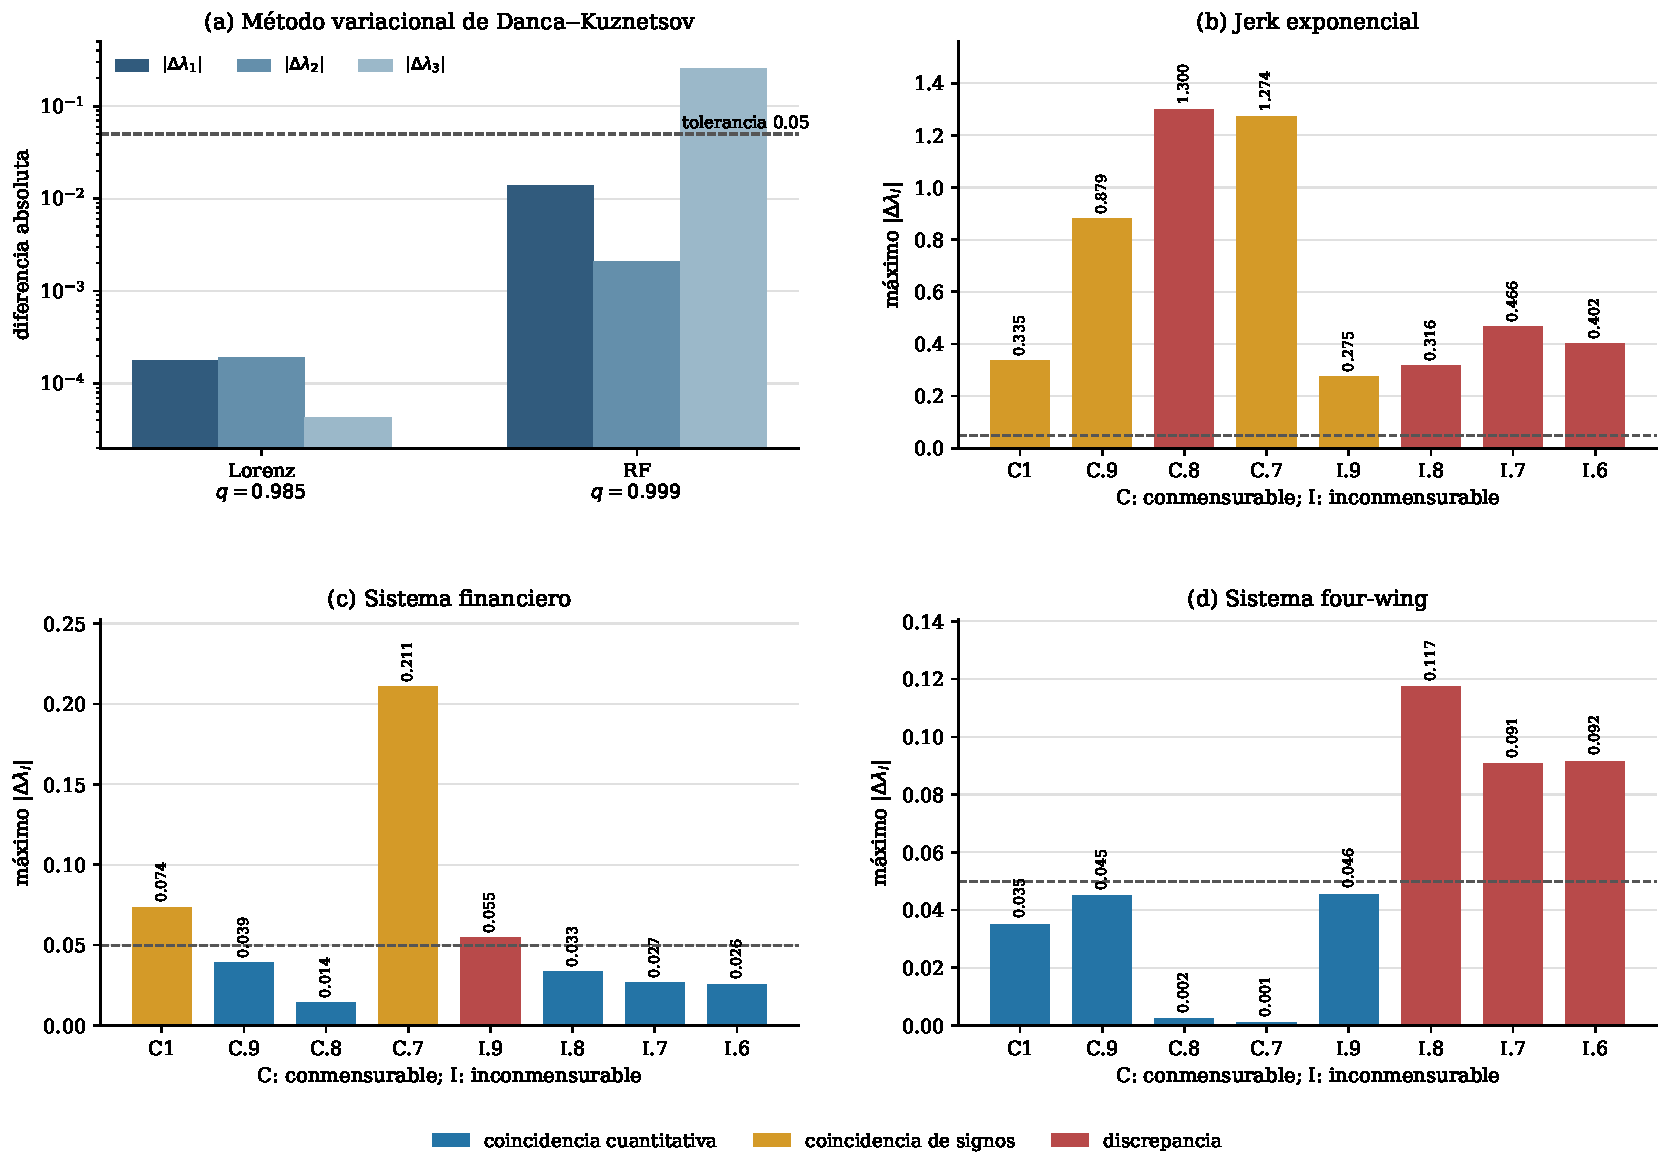
\includegraphics[width=0.96\linewidth]{figures/nonchua_benchmarks/lyapunov_validation_overview.pdf}
\caption{Comparación numérica de los exponentes publicados y calculados. El
panel DK2018 muestra los dos casos variacionales; los paneles Fischer resumen
el error máximo por fila y distinguen coincidencias cuantitativas, apoyo por
patrón de signos y discrepancias.}
\label{fig:nonchua-lyapunov-validation}
\end{hafocommonfigure}

\subsection{Alcance de las conclusiones dinámicas}

Los exponentes de Lorenz, RF, jerk, financiero y four-wing verifican rutas de
cálculo bajo configuraciones publicadas. No sustituyen las etapas de
localización y ocultedad: falta una semilla obtenida de las ecuaciones, una
continuación hasta el sistema objetivo, la identificación de una nube o ciclo
recurrente, la robustez frente a paso y método, y el análisis de vecindades de
todos los equilibrios. Por esta razón, ninguno de estos cinco sistemas se añade
a la lista de atractores ocultos localizados. La evidencia de mayor nivel en el
conjunto no Chua corresponde a Kalman--Fitts, MAVPD y PLL, cuyos resultados y
figuras se presentan en la sección de sistemas enteros.
